\section{Background}\label{Background}

\subsection{Datacenter Networking Solutions}

The problem of TCP processing overheads is not a new problem, and it is a 
problem that will likely never be completely solved. Simply using Linux and
accepting the performance loss is simply not an option for datacenter 
applications. Several alternatives have been proposed.

\paragraph{Kernel Bypass.} 

The simplest solution to kernel network stack overheads is to simply bypass
it entirely. Arrakis \cite{peter:arrakis} showed that if we remove the kernel
from the packet processing path and do everything from user-level, the time 
required to process one packet can be up to 16 times less. As userspace network
stacks already existed \cite{lwip}, this solution found immediate success out of
the box with solutions like mtcp\cite{mtcp}. For datacenter applications, \
regular kernel bypass is frowned upon, as it takes control of certain operations
away from the kernel and gives the application more freedom to interact with the
network, typically interacting poorly with congestion control policies. As a 
result, protected kernel bypass solutions such as IX \cite{belay:ix} were 
proposed, which provide greater protection with some performance tradeoffs. 

\paragraph{Hardware Offload.}

The current trend for addressing and accelerating packet processing is towards
hardware offload\cite{chelsio_toe}. Many NICs already support some kind of 
fixed-function offload like checksum or segmentation, but the research community
has been pushing for more. Solutions such as offloading the entire data path to 
the NIC have been proposed, but have had difficulty being adopted due to how 
difficult and slow development is, for both creating the initial implementation 
and evolving it to meet future datacenter needs. 

\subsection{TCP acceleration as a service (TAS)}

In an attempt to combine the performance benefits of kernel bypass, the 
protection of separated applications and network stacks, and the flexibility of
a software-only solution, TCP acceleration as a service has been proposed (TAS).

TAS was designed with a number of goals in mind. Most importantly, it provides
efficient and scalable packet processing. The network stack is optimized to use 
the least amount of cycles while generating the smallest amount of network time,
while also maintaining the ability to scale to high numbers of connections. 
TAS also maintains highly predictable performance at datacenter scale, an 
important quality for datacenter management tools and user quality of service.
TAS does all this while maintaining strict policy requirements placed upon the
applications and scaling CPU usage based on need. 
 
One key idea that TAS leverages is that the TCP stack can be divided into two 
parts: a slow path and a fast path. The slow path handles typical control and 
time intensive operations like connection setup/teardown, timeouts, and out of 
order packets, whereas the fast path handles common-case data packets. Figure 
\ref{fig:splittcp} shows the general idea of TAS; the user's application use an 
unmodified POSIX API to talk to a user-level TCP library. The fast path can 
directly read from and write to the network card through DPDK \cite{dpdk}; when 
data packets arrive or need to be sent out, the fast path directly communicates 
with the user-level library; when it gets packets that have to be handled by the
slow path (such as SYN packets), the packet is offloaded to it through shared 
memory.

\begin{figure}
\centering
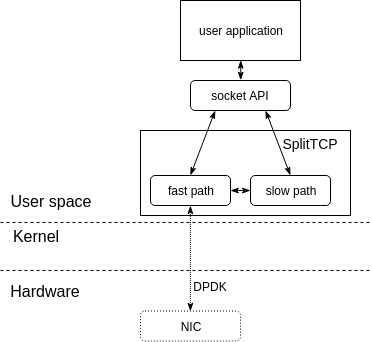
\includegraphics[width=0.7\columnwidth]{figures/splittcp_default.png}
\caption{The idea behind TAS is split network operations between a slow and a fast path, both in user level, completely
avoiding the kernel.}
\label{fig:splittcp}
\end{figure}

\subsection{Linux Compatability}

While TAS provides a lot of benefits, it would be too labor intensive to match 
the full functionality of the Linux network stack. Because TAS is implemented
entirely in userspace, it makes it hard to interact directly with the Linux 
kernel. However, solutions exist to integrate TAS with Linux in a more creative
way. By utilizing virtual network interfaces with Linux, we can appear to be the
network interacting with Linux, spoofing packets and observing Linux's behavior 
to gain knowledge and functionality from Linux. 

\subsection{TAP devices}

One of the tools used in this work was TUN/TAP devices. These are virtual network devices that are purely software 
(hence the ``virtual''). These devices mimic a physical NIC, the only difference is that instead of receiving/sending
data to the outside through a wire/radio waves, it is done so to a buffer in kernel space that an application can read/write
through the POSIX file API. Figure \ref{fig:tap} has a basic representation of both concepts: when using a regular (wired)
NIC, the kernel gets calls from user space, and sends/receives from a physical device. When using a TUN/TAP device, the data is
read/written to a buffer in kernel, and an application in user space can capture and write raw network data to and from it, 
emulating a real outside connection.

The different between TUN and TAP is the network layer in which they work. TUN devices work in layer 3 (IP packets), while TAP
devices work in layer 2 (ethernet frames).


\begin{figure}
\centering
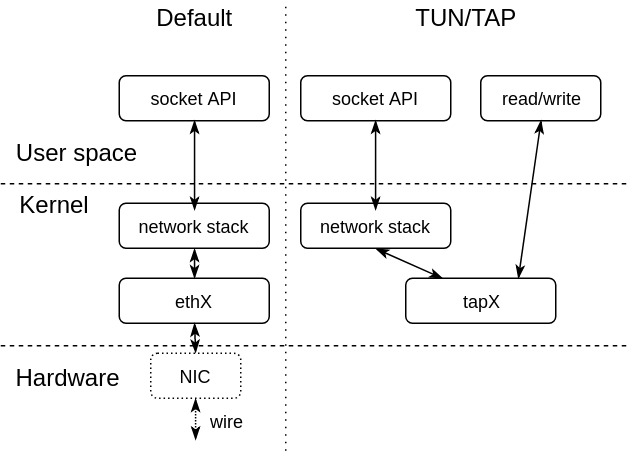
\includegraphics[width=0.7\columnwidth]{figures/tap_diag.png}
\caption{The difference between the usage of a regular NIC from a TUN/TAP device. In the latter the data is not sent to the
outside, but stored as raw data in a kernel space buffer which an application can read and write to.}
\label{fig:tap}
\end{figure}
